\documentclass{standalone}
\usepackage{tikz}
\usepackage{xcolor}
\usetikzlibrary{intersections}

\begin{document}
	
	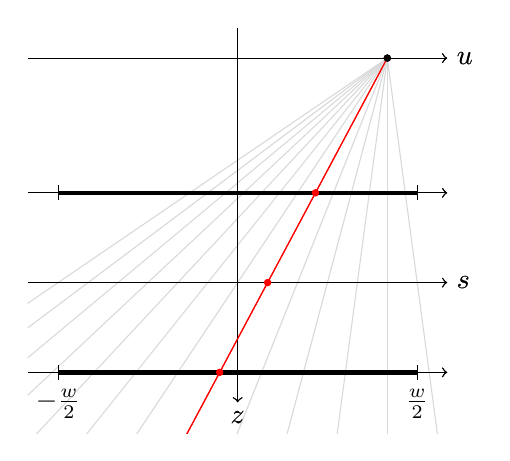
\begin{tikzpicture}[scale = 0.19,
						one end extended/.style = {shorten <= -#1},
	 					one end extended/.default = 1cm,
	 					]
	
		\colorlet{lightgray}{gray!30}
		
		% Top and bottom layer planes
		\draw[->, name path = bottomLayer] (-14, -6) -- (14, -6);
		\draw[->, name path = topLayer] (-14, 6) -- (14, 6);
					
		% Camera plane
		\draw[->] (-14, 15) -- (14, 15);
		\node[right] at (14, 15) {$u$};
		
		% Sensor plane
		\draw[<-, name path = sensor] (14, 0) -- (-14, 0);
		\node[right] at (14, 0) {$s$};
			
		% Camera position marker
		\coordinate (cameraCenter) at (10, 15);
		\fill[black] (cameraCenter) circle[radius = 0.25];
				
		\draw[ultra thick] (-12, -6) -- (12, -6);
		\draw[ultra thick] (-12, 6) -- (12, 6);
				
		% z-axis
		\draw[->] (0, 15 + 2) -- (0, -8);
		\node[below] at (0, -8) {$z$};
		
		% Save current bounding box to clip light rays
		\coordinate (NE) at (current bounding box.north east);
		\coordinate (SW) at (current bounding box.south west);
		\clip (SW) rectangle (NE);
		
		% Rays and intersections
		\coordinate (s0) at (-12, 0);
		\coordinate (s1) at (-10, 0);
		\coordinate (s2) at (-8, 0);
		\coordinate (s3) at (-6, 0);
		\coordinate (s4) at (-4, 0);
		\coordinate (s5) at (-2, 0);
		\coordinate (s6) at (0, 0);
		\coordinate (s7) at (2, 0);
		\coordinate (s8) at (4, 0);
		\coordinate (s9) at (6, 0);
		\coordinate (s10) at (8, 0);
		\coordinate (s11) at (10, 0);
		\coordinate (s12) at (12, 0);
		
		\draw[one end extended = 10cm, lightgray] (s0) -- (cameraCenter);
		\draw[one end extended = 10cm, lightgray] (s1) -- (cameraCenter);
		\draw[one end extended = 10cm, lightgray] (s2) -- (cameraCenter);
		\draw[one end extended = 10cm, lightgray] (s3) -- (cameraCenter);
		\draw[one end extended = 10cm, lightgray] (s4) -- (cameraCenter);
		\draw[one end extended = 10cm, lightgray] (s5) -- (cameraCenter);
		\draw[one end extended = 10cm, lightgray] (s6) -- (cameraCenter);
		\draw[one end extended = 10cm, red, name path = ray] (s7) -- (cameraCenter);
		\draw[one end extended = 10cm, lightgray] (s8) -- (cameraCenter);
		\draw[one end extended = 10cm, lightgray] (s9) -- (cameraCenter);
		\draw[one end extended = 10cm, lightgray] (s10) -- (cameraCenter);
		\draw[one end extended = 10cm, lightgray] (s11) -- (cameraCenter);
		\draw[one end extended = 10cm, lightgray] (s12) -- (cameraCenter);
		
		% Draw lines of coordinate system again on top of rays
		\draw[->] (-14, -6) -- (14, -6);
		\draw[->] (-14, 6) -- (14, 6);
		\draw[->] (-14, 15) -- (14, 15);
		\node[right] at (14, 15) {$u$};
		\draw[<-] (14, 0) -- (-14, 0);
		\node[right] at (14, 0) {$s$};
		\draw[ultra thick] (-12, -6) -- (12, -6);
		\draw[ultra thick] (-12, 6) -- (12, 6);
		\draw[->] (0, 15 + 2) -- (0, -8);
		\node[below] at (0, -8) {$z$};
		
		\draw[one end extended = 10cm, red, name path = ray] (s7) -- (cameraCenter);
		\fill[black] (cameraCenter) circle[radius = 0.25];
		
		% Intersection markers
		\fill[red] (-1.2, -6) circle[radius = 0.25];
		\fill[red] (2, 0) circle[radius = 0.25];
		\fill[red] (5.2, 6) circle[radius = 0.25];
							
		% Width markers
		\draw (-12, -0.5 + 6) -- (-12, 0.5 + 6);
		\draw (12, -0.5 + 6) -- (12, 0.5 + 6);
		\draw (-12, -0.5 - 6) -- (-12, 0.5 - 6);
		\draw (12, -0.5 - 6) -- (12, 0.5 - 6);
		\node[below] at (-12, -0.5 - 6) {$-\frac{w}{2}$};
		\node[below] at (12, -0.5 - 6) {$\frac{w}{2}$};
		
	\end{tikzpicture}
	
\end{document}